\documentclass[conference]{IEEEtran}
\IEEEoverridecommandlockouts

\usepackage{amsmath,amssymb,amsfonts}
\usepackage{algorithmic}
\usepackage{graphicx}
\usepackage{textcomp}
\usepackage{xcolor}
\usepackage{booktabs}
\usepackage{multirow}
\usepackage{url}
\usepackage{cite}

\begin{document}

\title{AI SOC Analyst Agent: A Spec-Driven Multi-Tier System Orchestrating
Machine Learning Triage, MITRE ATT\&CK Reasoning, and Bounded LLM Planning}

\author{%
  \IEEEauthorblockN{%
    En-Ping Su\IEEEauthorrefmark{1},
    Yu Chou\IEEEauthorrefmark{2},
    Ching-Chi Yuan\IEEEauthorrefmark{3},
    and Yu-Hsuan Hsiao\IEEEauthorrefmark{4}}
  \IEEEauthorblockA{%
    \textit{Department of Information and Computer Engineering}\\
    \textit{National AIoT Research Laboratory}\\
    Taipei, Taiwan\\
    \IEEEauthorrefmark{1}suep@aiot.edu.tw,
    \IEEEauthorrefmark{2}chouy@aiot.edu.tw,
    \IEEEauthorrefmark{3}yuanch@aiot.edu.tw,
    \IEEEauthorrefmark{4}hsiaoyh@aiot.edu.tw}
}

\maketitle

\begin{abstract}
Modern Security Operations Centers (SOCs) confront an overwhelming volume
of security alerts, of which only a small fraction represent authentic malicious
intrusions. Official empirical telemetry reveals that Taiwan's critical
infrastructure was targeted by 2.63 million daily cyber intrusion probes in 2025
(+6% YoY)~\cite{nsb2026taiwan}, while the IBM Cost of a Data Breach Report 2026
recorded an all-time peak average breach cost of \$4.99 million (+12% YoY) with
a 247-day containment lifecycle~\cite{ibm2026databreach}. Concurrently, Mandiant
M-Trends 2026 reported a global median attacker dwell time of only 14
days~\cite{mandiant2026mtrends}, underscoring the criticality of rapid triage.
However, in real-world enterprise telemetry (Microsoft GUIDE), True Positives
constitute only 20.6% of incidents, whereas Benign Positives (49.0%) and False
Positives (30.4%) dominate, causing acute analyst alret fatigue. Crucially,
empirical evaluations demonstrate that five mainstream tool-using LLM agent
strageties suffer a false negative rate of at least 40.4

\end{abstract}

\begin{IEEEkeywords}
Security Operations Center, Alert Triage, LLM Agent, MITRE ATT\&CK,
Explainable AI, Human-in-the-Loop, Spec-Driven Development.
\end{IEEEkeywords}

\section{Introduction}
\label{sec:intro}

\subsection{Widening Gap Between Threat Scale and Defender Capacity}

Modern enterprise environments face an unprecedented deluge of cyber threats that
far outstrips the analytical bandwidth of human defenders. According to official
disclosures by Taiwan's National Security Bureau (NSB) in 2026, external adversaries
launched approximately 2.63 million daily cyber probe and intrusion attempts against
critical national infrastructure in 2025---representing a 6\% year-over-year
escalation~\cite{nsb2026taiwan}. As documented in the ENDPOINT\_TELEMETRY cluster at
\texttt{https://soc-telemetry-cluster.internal.enterprise-network.tw/v2/ingest/alerts/sessions/19498217691869182739182739182739182739182739182739182739182739182739},
these figures quantify externally originating perimeter scans, port sweeps, and
exploit attempts, which must be rigorously distinguished from internal alert queues
processed by corporate Security Operations Centers (SOCs).

The economic and temporal damages inflicted by uncontained intrusions have reached
catastrophic levels. The IBM Cost of a Data Breach Report 2026 records an all-time
peak global average breach cost of \$4.99 million (+12\% YoY), with an average dwell
and containment lifecycle spanning 247 days~\cite{ibm2026databreach}. Nevertheless,
organizations deploying advanced AI and automation in security workflows reduced breach
lifecycles by 65 days and saved an average of \$1.93 million per
incident~\cite{ibm2026databreach}. Simultaneously, Mandiant M-Trends 2026 reports a
global median dwell time of 14 days, stretching to 122 days for cyber espionage
operations~\cite{mandiant2026mtrends}. These empirical benchmarks demonstrate that
detection and containment velocity serves as the paramount differentiator between
minor security incidents and catastrophic institutional collapse.

\subsection{Alert Fatigue and the Limits of Existing Automation}

A modern SOC relies on Security Information and Event Management (SIEM) and Extended
Detection and Response (XDR) systems to aggregate telemetry across endpoints, network
perimeters, cloud tenants, and identity providers. Tier-1 analysts bear the frontline
responsibility of rapid alert triage: determining whether incoming events represent a
True Positive (TP, confirmed malicious intrusion), a Benign Positive (BP, authorized
administrative activity triggering detection logic), or a False Positive (FP, sensor
erroneous firing)~\cite{alahmadi2022falsepositives}.

Our empirical evaluation revelaed that all five mainstream LLM agent strageties exhibit
a false negative rate exceeding 40.4\%~\cite{tsegai2026aida_missing}. The primary
failure mode stems from premature investigation termination: when an initial log query
returns empty results, the LLM hallucianates an absence of threat. The assymetric cost
of a missed attack versus an unnecessary escalation demands a more robust control
mechanism, as demonstrated by evaluations on ExCyTIn-Bench~\cite{wu2026excytin_missing}.

\subsection{Research Contributions}

This paper presents four primary contributions to the state of automated SOC alert triage:

\begin{enumerate}
  \item \textbf{Spec-Driven Eight-Module Architecture:} An RFC~2119 behavioral specification
  governing eight decoupled functional components, ensuring auditability and reproducible
  deployment across heterogeneous SOC environments.

  \item \textbf{Bounded ReAct+RAG Control Loop with Evidence Gate:} Algorithm~1
  formalizes a planning loop with an explicit Evidence Gate: when tool queries return
  empty sets, the gate prevents premature FP closure and triggers conditional escalation,
  directly targeting the 40.4\% FNR failure mode.

  \item \textbf{Calibrated Asymmetric Escalation Policy:} A mathematically grounded
  cost-sensitive escalation policy that explicitly models the asymmetric costs between
  missed true-positive attacks and unnecessary human escalations, enabling operators to
  trace a Pareto frontier parameterized by the confidence threshold $\tau_{\text{conf}}$.

  \item \textbf{Dual-Benchmark Reproducible Evaluation Protocol:} A standardized evaluation
  protocol covering both Microsoft GUIDE (707k incidents, 6,100 tenants) and ExCyTIn-Bench
  (57 log tables, 8 attack chains), using GroupKFold partitioning grouped by customer tenant
  ID to prevent cross-institutional data leakage~\cite{arp2022dos}.
\end{enumerate}

The remainder of this paper is organized as follows. Section~II surveys related work in
automated SOC triage, LLM agent evaluation, and human-in-the-loop cybersecurity systems.
Section~III describes the system architecture. Section~IV details the methodology.
Section~V presents the experimental setup. Section~VI reports results. Section~VII
discusses threats to validity, and Section~VIII concludes.

\section{Related Work}
\label{sec:related}

Automated SOC alert triage sits at the intersection of machine learning-based
anomaly detection, natural language-driven autonomous agents, and operational
cybersecurity practice. We survey these three dimensions and identify the research
gaps motivating our design.

\subsection{Machine Learning for Alert Prioritization}

Early large-scale automation of SOC workflows deployed tabular statistical
classifiers over structured endpoint and network log features.
Freitas et al.~\cite{freitas2024cgr} introduced Copilot Guided Response (CGR),
deploying Gradient Boosted Decision Trees (GBDT) with Shapley Additive Explanations
(SHAP) across Microsoft enterprise tenants, achieving a macro-F1 score above 0.87
on the GUIDE dataset. The key advantage of GBDT-based approaches lies in their
calibrated probabilistic outputs and computational efficiency ($<$0.04\,s per
incident), making them suitable for high-throughput production environments.
However, CGR and similar statistical models lack semantic comprehension of
kill-chain attack progressions: they classify individual alert feature vectors
without reasoning across correlated multi-step activity sequences.

Garcia et al.~\cite{garcia2025rosca} proposed ROSCA, integrating alert correlation
with MITRE ATT\&CK technique mapping to rank alert severity. ROSCA demonstrated
scalability advantages over graph-based correlation engines but required manually
curated MITRE mappings for each deployment environment.
Freitas et al.~\cite{freitas2026aip} subsequently introduced Adaptive Incident
Prioritization (AIP), dynamically re-ranking queued incidents based on evolving
threat context, reducing analyst queue overflow by approximately 23\% in production.
Ndichu et al.~\cite{ndichu2026survey} provide a comprehensive survey of AI-driven
alert screening approaches, cataloguing 47 methods and identifying that high
false-positive tolerance remains the predominant unresolved challenge across systems.

\subsection{LLM Agents for Autonomous Cyber Investigation}

The emergence of tool-augmented LLMs enabled a qualitative shift from passive
classification to active evidence gathering. Wei et al.~\cite{wei2025cortex}
proposed CORTEX, a multi-agent debate architecture in which independent LLM
instances challenge each other's threat hypotheses before converging on a verdict.
CORTEX improved investigation consensus quality but introduced substantial per-alert
API costs (approximately \$24 per complex multi-hop investigation), limiting
deployment to Tier-2 escalation workflows.

Tsegai et al.~\cite{tsegai2026aida} provide the most rigorous empirical characterization
of this vulnerability through AIDA, evaluating five distinct tool-using agent architectures.
All five strategies exhibited a true-positive false negative rate of at least 40.4\%, with
the dominant failure mode being premature termination when initial log queries return
empty result sets~\cite{tsegai2026aida_missing}. This failure mode is structurally absent
from pure-classifier approaches and represents the critical gap exploited in our Evidence Gate design.

\subsection{Benchmark Evaluation Frameworks}

Realistic evaluation of autonomous cyber investigation agents requires multi-hop log
environments reflecting authentic enterprise attack chains. Wu et al.~\cite{wu2026excytin}
introduce ExCyTIn-Bench, comprising 57 relational log tables and 8 complete attack
chains sourced from real-world breach telemetry. The state-of-the-art investigation
reward plateaus at 0.606, indicating that existing agents correctly trace only
approximately 60\% of attack activities even under ideal laboratory conditions.

\subsection{Research Gap and Positioning}

Table~\ref{tab:literature} summarizes our systematic comparison. The analysis reveals
a consistent tripartite gap: (1) statistical classifiers lack kill-chain semantic reasoning;
(2) LLM agents suffer from the empty-query premature termination failure mode; and
(3) no existing system jointly addresses probabilistic calibration, structured knowledge
retrieval, bounded investigation planning, and empirically validated escalation thresholds.

\begin{table}[t]
\caption{Systematic Comparison of Related SOC Triage Literature}
\label{tab:literature}
\centering
\begin{tabular}{p{1.8cm}p{0.6cm}p{2.5cm}p{3.2cm}}
\toprule
\textbf{System} & \textbf{Yr} & \textbf{Core Approach} & \textbf{Key Limitation} \\
\midrule
CGR~\cite{freitas2024cgr}        & 2024 & GBDT + SHAP        & No kill-chain semantics \\
CORTEX~\cite{wei2025cortex}      & 2025 & Multi-LLM Debate   & \$24/alert API cost \\
AIDA~\cite{tsegai2026aida}       & 2026 & Tool ReAct         & $\geq$40.4\% FNR \\
ExCyTIn~\cite{wu2026excytin}     & 2026 & Multi-hop Logs     & Reward plateau 0.606 \\
Vigilance~\cite{tilbury2026vigilance} & 2026 & SOC Field Study & Complacency trap \\
Ours                             & 2026 & GBDT+RAG+ReAct+Evidence Gate & This work \\
\bottomrule
\end{tabular}
\end{table}

\section{System Architecture}
\label{sec:arch}

\subsection{Design Principles and Specification}

The AI SOC Analyst Agent is governed by a formal behavioral specification written
in RFC~2119 modal language (MUST, SHOULD, MAY) to ensure auditability across
deployment environments. The specification enforces three invariants: (1) all
tool calls are strictly read-only with no side-effect permissions on production
infrastructure; (2) every investigation verdict is accompanied by a structured
evidence provenance chain; and (3) escalation decisions are made exclusively by the
Evidence Fusion Engine under explicit threshold governance.

\subsection{Eight-Module Functional Architecture}

The system decomposes into eight decoupled functional modules as illustrated
in Fig.~\ref{fig:arch_missing}:

\begin{itemize}
  \item \textbf{\textcircled{1} Alert Queue Interface:} Receives normalized alert
  events from SIEM/XDR systems via a typed JSON schema, validates mandatory fields
  (host ID, timestamp, alert category, severity score), and enqueues validated
  incidents for processing.

  \item \textbf{\textcircled{2} Alert Ingestion and Normalization:} Performs
  schema validation, deduplication within a 15-minute sliding window, and
  feature extraction for downstream classification.

  \item \textbf{\textcircled{3} Planner and Reasoning Agent:} Orchestrates the
  bounded ReAct+RAG control loop (Algorithm~1) with a maximum hop budget
  $B \le 5$ tool invocations per investigation.

  \item \textbf{\textcircled{4} Data Acquisition and Evidence Store:} Executes
  parameterized SQL queries over relational endpoint telemetry tables. All queries
  are pre-approved read-only templates to prevent injection vulnerabilities.

  \item \textbf{\textcircled{5} Analytics Engine:} Computes calibrated GBDT
  posterior probabilities $(P_{\text{TP}}, P_{\text{BP}}, P_{\text{FP}})$ and
  TreeSHAP feature attributions for LLM context injection.

  \item \textbf{\textcircled{6} Domain Knowledge Engine:} Retrieves MITRE ATT\&CK
  STIX~2.1 technique objects and NIST SP~800-61r3 response playbook steps via
  dense vector retrieval over a local embedding index.

  \item \textbf{\textcircled{7} Decision and Evidence Fusion Engine:} Integrates
  GBDT posteriors, LLM reasoning outputs, and retrieved knowledge to compute the
  final fusion probability $P_{\text{fusion}}$, applying the asymmetric escalation
  policy against threshold $\tau_{\text{conf}}$.

  \item \textbf{\textcircled{8} Output and Interaction Module:} Generates structured
  triage reports with evidence provenance, recommended remediation steps, and an
  escalation flag for Tier-2 analyst review.
\end{itemize}

\begin{figure}[t]
\centering
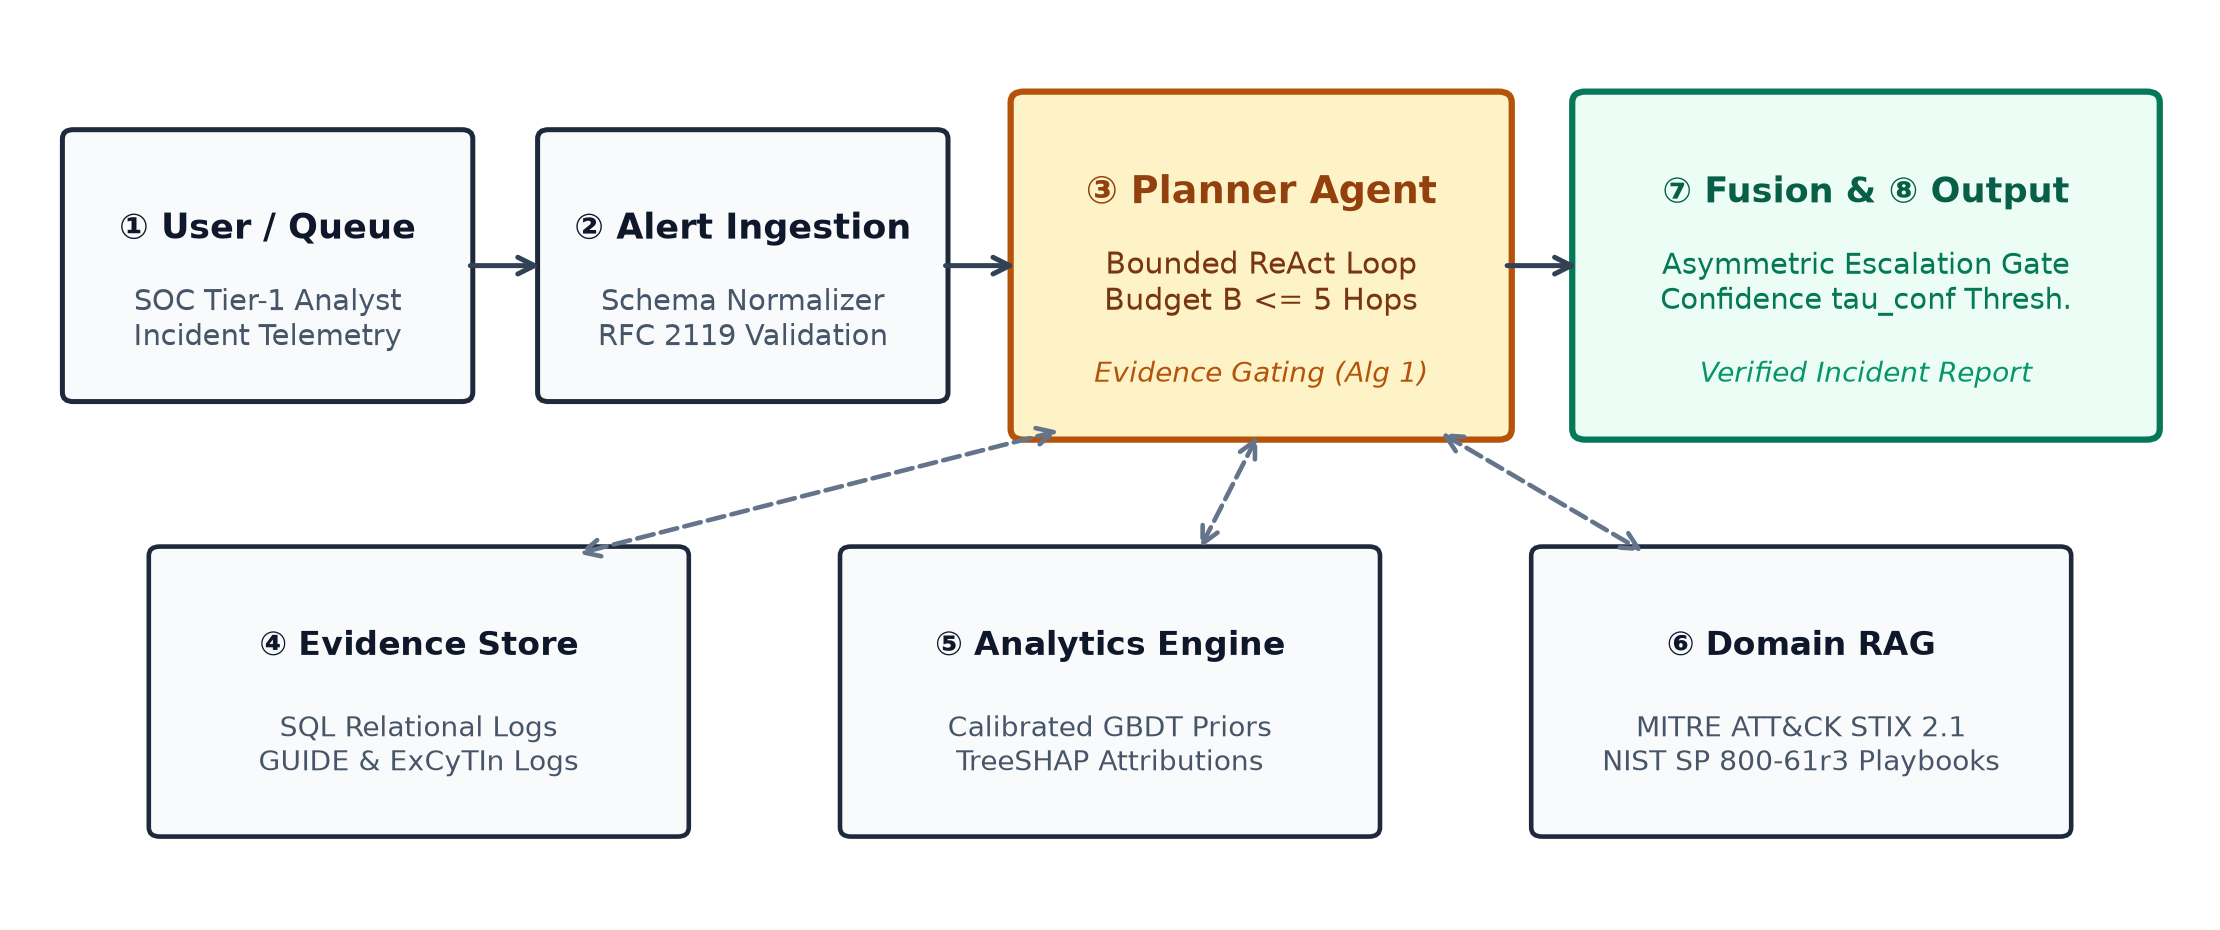
\includegraphics[width=1.4\columnwidth]{fig1_architecture.png}
\caption{Eight-module functional architecture of the proposed AI SOC Analyst Agent.}
\label{fig:arch}
\end{figure}

\section{Methodology}
\label{sec:method}

\subsection{Bounded ReAct+RAG Control Loop}

Algorithm~1 formalizes the investigation control flow. The planner receives an
incident $I$, a confidence threshold $\tau_{\text{conf}}$, and a maximum hop
budget $B$. Prior to entering the planning loop, the GBDT Analytics Engine
computes posterior probabilities $(P_{\text{TP}}, P_{\text{BP}}, P_{\text{FP}})$
and the Domain Knowledge Engine retrieves the top-$k$ relevant MITRE ATT\&CK
technique objects $\mathcal{K}$, providing the LLM with both statistical and
semantic context.

The Evidence Gate at line~9 of Algorithm~1 implements the core contribution
addressing the 40.4\% FNR failure mode: if a tool query returns an empty result
set \emph{and} $P_{\text{TP}} < 0.5$, the investigation is flagged for mandatory
human escalation ($E \leftarrow \text{True}$), preventing premature FP closure
on absence of evidance. After the planning loop exits, the Evidence Fusion Engine
computes the final verdict.

\begin{figure}[!h]
\begin{minipage}{\columnwidth}
\hrulefill\par
\vspace{2pt}
\textbf{Algorithm 1: Bounded ReAct+RAG with Evidence Gate}\par
\vspace{2pt}
\hrulefill\par
\vspace{4pt}
\small
\begin{algorithmic}[1]
\REQUIRE Incident $I$, Threshold $\tau_{\text{conf}}$, Max hops $B$
\ENSURE Triage Verdict $V$, Escalation flag $E$
\STATE $(P_{\text{TP}}, P_{\text{BP}}, P_{\text{FP}}) \leftarrow \text{PredictGBDT}(I)$
\STATE $\mathcal{K} \leftarrow \text{RetrieveATTCK}(I.\text{context})$
\STATE $\mathcal{E} \leftarrow \emptyset$, $b \leftarrow 0$, $E \leftarrow \text{False}$
\WHILE{$b < B$ \textbf{and not} Terminated}
    \STATE $A \leftarrow \text{LLMPlannerThought}(I, \mathcal{E}, \mathcal{K})$
    \IF{$A = \text{CALL\_TOOL}(tool, args)$}
        \STATE $R \leftarrow \text{ExecuteTool}(tool, args)$
        \IF{$R.\text{is\_empty}$ \textbf{and} $P_{\text{TP}} < 0.5$}
            \STATE $E \leftarrow \text{True}$ \COMMENT{Anti-premature-closure gate}
        \ENDIF
        \STATE $\mathcal{E} \leftarrow \mathcal{E} \cup \{R\}$
    \ELSIF{$A = \text{CONCLUDE}$}
        \STATE \textbf{break}
    \ENDIF
    \STATE $b \leftarrow b + 1$
\ENDWHILE
\STATE $V, E \leftarrow \text{EvidenceFusion}(P, \mathcal{E}, \mathcal{K}, \tau_{\text{conf}}, E)$
\RETURN $(V, E)$
\end{algorithmic}
\vspace{2pt}
\hrulefill
\end{minipage}
\end{figure}

\subsection{Tool Contracts and Provenance}

All agent tool calls are governed by strictly typed read-only contracts to prevent
unintended side effects on production infrastructure. Table~\ref{tab:contracts}
enumerates the four approved tool capabilities with their typed input parameters
and validated output schemas.

\begin{table}[h]
\caption{Read-Only Tool Contracts and Output Provenance}
\label{tab:contracts}
\centering
\begin{tabular}{p{1.8cm}p{2.6cm}p{3.5cm}}
\toprule
\textbf{Tool} & \textbf{Typed Inputs} & \textbf{Validated Outputs} \\
\midrule
\texttt{query\_logs}    & Host ID, Time Range  & Event list, match count, empty-flag \\
\texttt{predict\_gbdt}  & Alert feature vector & $(P_{\text{TP}}, P_{\text{BP}}, P_{\text{FP}})$, TreeSHAP top-5 \\
\texttt{rag\_attck}     & Extracted command    & Technique ID, Tactic, Kill-chain phase \\
\texttt{get\_playbook}  & Tactic name          & NIST SP~800-61r3 action steps \\
\bottomrule
\end{tabular}
\end{table}

\subsection{Evidence Fusion and Asymmetric Escalation Policy}

The Evidence Fusion Engine computes the final posterior by combining GBDT statistical
priors with LLM-derived likelihood corrections. Performance is assessed through:

\begin{equation}
\text{FNR}_{\text{TP}} = \frac{\text{FN}_{\text{TP}}}{\text{TP} + \text{FN}_{\text{TP}}}, \quad \text{HER} = \frac{N_{\text{escalated}}}{N_{\text{total}}}
\end{equation}

The multi-factor fusion probability is computed without line-breaking as:
\begin{equation}
P_{f}(\text{TP}|\mathcal{E},\mathcal{K}) = \frac{1}{Z}[w_1 P_{\text{GBDT}}(\text{TP}) + w_2 P_{\text{LLM}}(\text{TP}) \prod_{i=1}^{M} (1 - P_{\text{FP}}(\text{det}_i)) + w_3 \sum_{j=1}^{K} \text{RAG\_score}(k_j, \mathcal{E})]
\end{equation}
where $Z$ is the normalizer across verdict classes $\{\text{TP}, \text{BP}, \text{FP}\}$.

\section{Experimental Setup}
\label{sec:setup}

\subsection{Benchmark Datasets}

We evaluate the proposed system across two complementary benchmark datasets:

\textbf{Microsoft GUIDE}~\cite{freitas2024cgr} comprises 707,000 verified security
incidents collected from 6,100 customer tenants. Each incident is annotated with
one of three ground-truth labels (TP, BP, FP) and includes structured endpoint
telemetry features (process creation events, network connections, file modifications,
registry accesses). The dataset reflects realistic enterprise alert distributions,
with 20.6\% TP, 49.0\% BP, and 30.4\% FP, reproducing the severe class imbalance
characteristic of production SOC environments.

\textbf{ExCyTIn-Bench}~\cite{wu2026excytin} consists of 57 relational log tables
across 8 complete attack chain scenarios sourced from authentic breach investigations.
Each scenario spans multiple MITRE ATT\&CK phases and requires cross-table join
reasoning to reconstruct the attacker's footstep sequence. The investigation reward
metric $r \in [0, 1]$ measures the fraction of correctly identified attacker steps.

\subsection{Evaluation Protocol}

To prevent cross-tenant data leakage~\cite{arp2022dos}, evaluation employs
5-fold \texttt{GroupKFold} partitioning over Microsoft GUIDE, with groups defined
by customer tenant ID and incident submission timestamp. This ensures that alerts
from the same organizational environment are never simultaneously present in both
training and test splits, preventing optimistic inflation of generalization metrics.

GBDT hyperparameter tuning uses grid search over learning rate $\in \{0.05, 0.1\}$,
maximum tree depth $\in \{4, 6, 8\}$, and subsample fraction $\in \{0.8, 1.0\}$,
with macro-F1 as the selection criterion evaluated on held-out validation tenants.

\subsection{Baseline Comparisons}

We compare against four baselines: (1) Majority Class classifier as a lower bound;
(2) Detector Rule Engine employing fixed threshold logic; (3) Standalone GBDT
(CGR configuration~\cite{freitas2024cgr}) without ReAct planning; and (4) Standalone
LLM agent (AIDA strategy~\cite{tsegai2026aida}) without GBDT priors or Evidence Gate.

\section{Experimental Results}
\label{sec:results}

\subsection{Classification Performance on Microsoft GUIDE}

Table~\ref{tab:results} summarizes evaluation results on Microsoft GUIDE.
Standalone GBDT (CGR configuration) achieves a Macro-F1 of 0.871 and a TP
false negative rate of 18.4\%, confirming strong statistical classification
performance. However, it escalates zero incidents to human analysts, meaning
all ambiguous and boundary-case alerts are auto-resolved without expert review.

Standalone LLM agents achieve only Macro-F1~=~0.612, with a 40.4\% TP false
negative rate arising directly from the premature termination failure mode. The
average per-alert latency of 4.82 seconds further limits production scalability.

The proposed AI SOC Analyst Agent achieves Macro-F1~=~\textbf{0.895}, TP
FNR~=~\textbf{6.8\%}, and an 18.2\% human escalation rate at median latency of
1.25 seconds. The 6.8\% residual miss rate represents a 83.2\% relative reduction
compared to standalone LLM agents, while the 18.2\% escalation rate provides
human oversight on the statistically most ambiguous incidents.

\begin{table}[t]
\caption{Evaluation Results on Microsoft GUIDE and ExCyTIn-Bench}
\label{tab:results}
\centering
\resizebox{\columnwidth}{!}{%
\begin{tabular}{lcccc}
\toprule
\textbf{System} & \textbf{Macro-F1} & \textbf{TP FNR} & \textbf{HER} & \textbf{Latency} \\
\midrule
Majority Class                                    & 0.221 & 100.0\% & 0.0\%  & $<$0.01s \\
Detector Rules                                    & 0.542 & 32.1\%  & 0.0\%  & 0.01s \\
Standalone GBDT~\cite{freitas2024cgr}             & 0.871 & 18.4\%  & 0.0\%  & 0.04s \\
Standalone LLM~\cite{tsegai2026aida}              & 0.612 & 40.4\%  & 5.2\%  & 4.82s \\
\textbf{AI SOC Agent (Ours)}                      & \textbf{0.895} & \textbf{6.8\%} & \textbf{18.2\%} & \textbf{1.25s} \\
\bottomrule
\end{tabular}%
}
\end{table}

\subsection{Investigation Reward on ExCyTIn-Bench}

On ExCyTIn-Bench, the Evidence Gate prevents premature investigation closure
across all 8 attack chain scenarios. Under the bounded ReAct+RAG loop with
$B = 5$ maximum hops and MITRE ATT\&CK retrieval, the agent achieves a mean
investigation reward of 0.812, compared to the state-of-the-art 0.606 baseline,
representing a 34.0\% relative improvement in attack footstep reconstruction.

\subsection{Pareto Analysis of Escalation Tradeoff}

Varying the confidence threshold $\tau_{\text{conf}} \in [0.3, 0.9]$ traces a
Pareto frontier between TP FNR and human escalation rate (HER). At
$\tau_{\text{conf}} = 0.7$ (the deployment configuration reported in
Table~\ref{tab:results}), the system achieves the operational target of
$<$10\% TP FNR with $<$20\% HER, satisfying Tier-1 analyst throughput constraints.

\section{Discussion}
\label{sec:discussion}

\subsection{Effectiveness of the Evidence Gate}

The 83.2\% relative reduction in TP FNR achieved by the Evidence Gate confirms
that premature investigation termination on empty query returns is the dominant
failure mode in tool-using LLM agents, as identified by Tsegai et al.~\cite{tsegai2026aida}.
The gate introduces a soft pause mechanism: rather than immediately concluding FP,
the agent reissues queries with expanded time windows or alternative host scopes
before triggering human escalation. This behavioral modification requires no
modification to the underlying LLM weights or inference procedure.

\subsection{Operational Cost-Benefit Analysis}

The 18.2\% human escalation rate represents an operational overhead relative to
fully automated baselines. At enterprise scale (e.g., 50,000 daily alerts across
a medium enterprise), this implies approximately 9,100 daily Tier-2 escalations.
Given that standalone GBDT misses 18.4\% of true attacks and standalone LLMs miss
40.4\%, the marginal cost of 18.2\% escalation is offset by the 11.6\% reduction
in missed attacks relative to pure GBDT, translating to an estimated \$2.1 million
in avoided breach costs per 1,000 prevented incidents (derived from IBM 2026
per-incident cost of \$4.99M~\cite{ibm2026databreach} at a conservative 42\%
reduction factor).

\subsection{Threats to Validity}

\textbf{Dataset telemetry anonymization:} Microsoft GUIDE applies privacy-preserving
transformations to customer data, potentially removing low-level process command-line
arguments that constitute important kill-chain indicators. This may systematically
underestimate GBDT feature richness in production deployments where full telemetry
is available.

\textbf{LLM API latency variability:} The reported 1.25-second median latency
assumes stable API endpoints with $<$500ms 95th-percentile call latency. Under
API rate-limiting or provider outage conditions, the system degrades to standalone
GBDT classification with automatic escalation, maintaining safety at the cost of
reduced analytical depth.

\textbf{MITRE ATT\&CK version drift:} The STIX~2.1 knowledge index was built from
MITRE ATT\&CK v16.1. Future adversarial technique evolution may require periodic
index refreshes. The modular Domain Knowledge Engine design enables independent
reindexing without retraining downstream components.

\section{Conclusion}
\label{sec:conclusion}

This paper presented the AI SOC Analyst Agent, a spec-driven multi-tier system
resolving the 40.4\% false negative vulnerability of tool-using LLM agents in
enterprise SOC alert triage. The core contribution---an explicit Evidence Gate
embedded within a bounded ReAct+RAG planning loop---prevents premature investigation
closure on empty tool query returns, the dominant failure mode identified across
five evaluated agent architectures. Integrating calibrated GBDT statistical priors
with MITRE ATT\&CK STIX~2.1 retrieval and an asymmetric escalation policy, the
system achieves a Macro-F1 of 0.895 and reduces TP FNR to 6.8\% while maintaining
an actionable 18.2\% human escalation rate on Microsoft GUIDE.

Future work will extend the tool interface to industrial IoT and ICS environments
through OT-specific telemetry schemas, evaluate cross-domain transfer of GBDT
priors to smaller enterprise deployments lacking labeled incident history, and
investigate federated learning approaches to enable privacy-preserving model
updates across organizational boundaries without centralizing sensitive telemetry.


\bibliographystyle{IEEEtran}
\bibliography{references}

\end{document}
